\subsection{Documentation for alamAPP}
\label{subsec:doc_alamAPP}
The alamAPP is a mobile-based test application developed to 
demonstrate the use of the alamSYS to external internet-connected 
devices, such as a smartphone application. It was created with the 
Dart-based Flutter SDK. The user interface and code snippets of how 
the alamSYS was used in the alamAPP are shown in this section. 
Furthermore, the full source code for the alamAPP is available 
in the GitHub repository listed in Appendix A of this paper.

\subsubsection{User Interface Showcase}
\label{subsubsec:alamAPP_UI}
This section displays the alamAPP's developed user interfaces. 
It should be noted that this application only highlights the 
alamSYS's two most important features, which are its ability 
to recommend which stocks to buy and which to sell. Additional 
enhancements to the application are discussed in Chapter 5 of 
this paper.
\\

% Insert Buy UI Here
The ability of the alamSYS to recommend stocks that are good to buy for the 
day is one of the key features of the alamSYS that is highlighted in the alamAPP. 
Users are able to see the list of stocks to buy as well as the necessary information 
about those stocks, including: (1) The last price as indicated below the stock symbol; 
and (2) The predicted price in 5 days as indicated in the green colored number at 
the rightmost part of the card listing. This is demonstrated in the alamAPP through 
the "Buy" Screen, presented in Figure \ref{fig:alamAPP_buy}. 
These details enable users to quickly assess a stock's potential return and choose 
from the list of stocks more wisely.
\begin{figure}[ht]
  \centering
  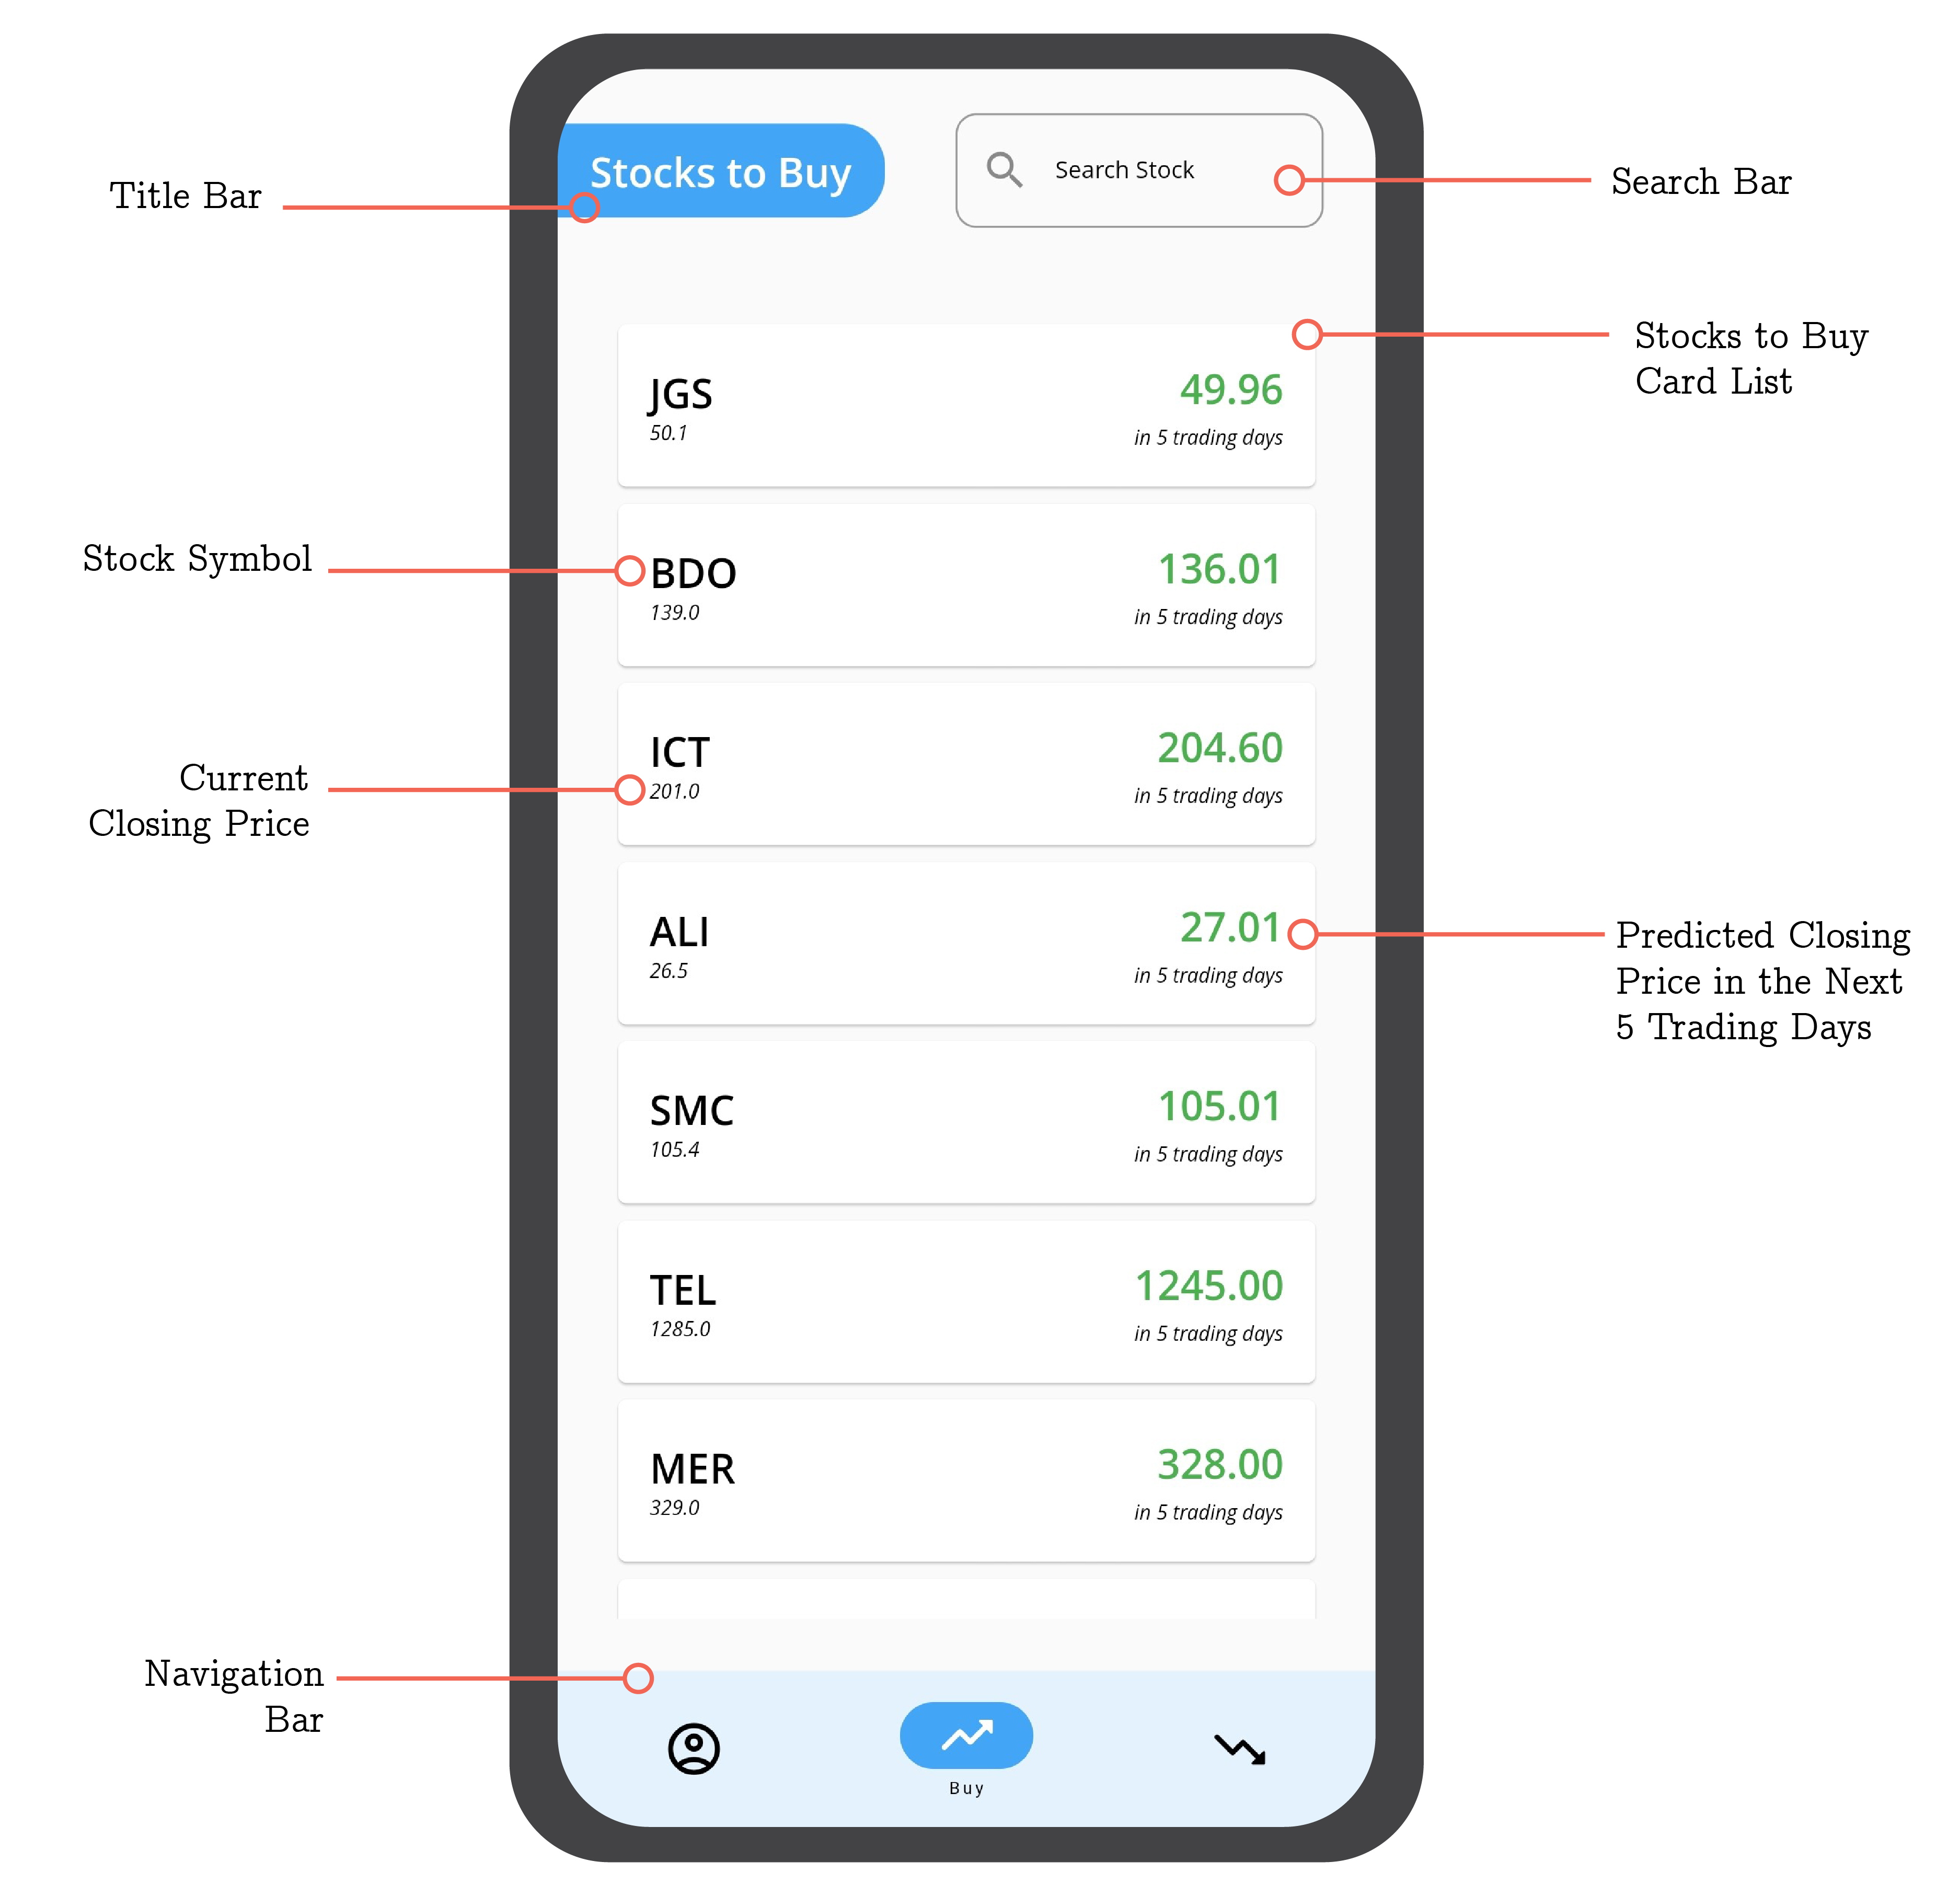
\includegraphics[height=0.40\textheight]{./assets/Chapter_4/mobile_ui/buy_ui.jpg}
  \caption{alamAPP "Buy" Screen}
  \label{fig:alamAPP_buy}
\end{figure}
\FloatBarrier


% Insert Sell UI Here
Another key feature of the alamSYS that is highlighted in the alamAPP is its ability to suggest 
stocks that must be sold for the day. This is demonstrated in the alamAPP by the "Sell" Screen, 
as shown in Figure \ref{fig:alamAPP_sell}, 
where users can see a list of which stocks to sell as well as the 
necessary information about those stocks, such as: (1) the last price as indicated below 
the stock symbol, and (2) the predicted price in 5 days as indicated in the red colored 
number at the rightmost part of the card listing. This information allows users to see the 
potential loss of the stock at a glance and better mitigate their risk.
\begin{figure}[ht]
  \centering
  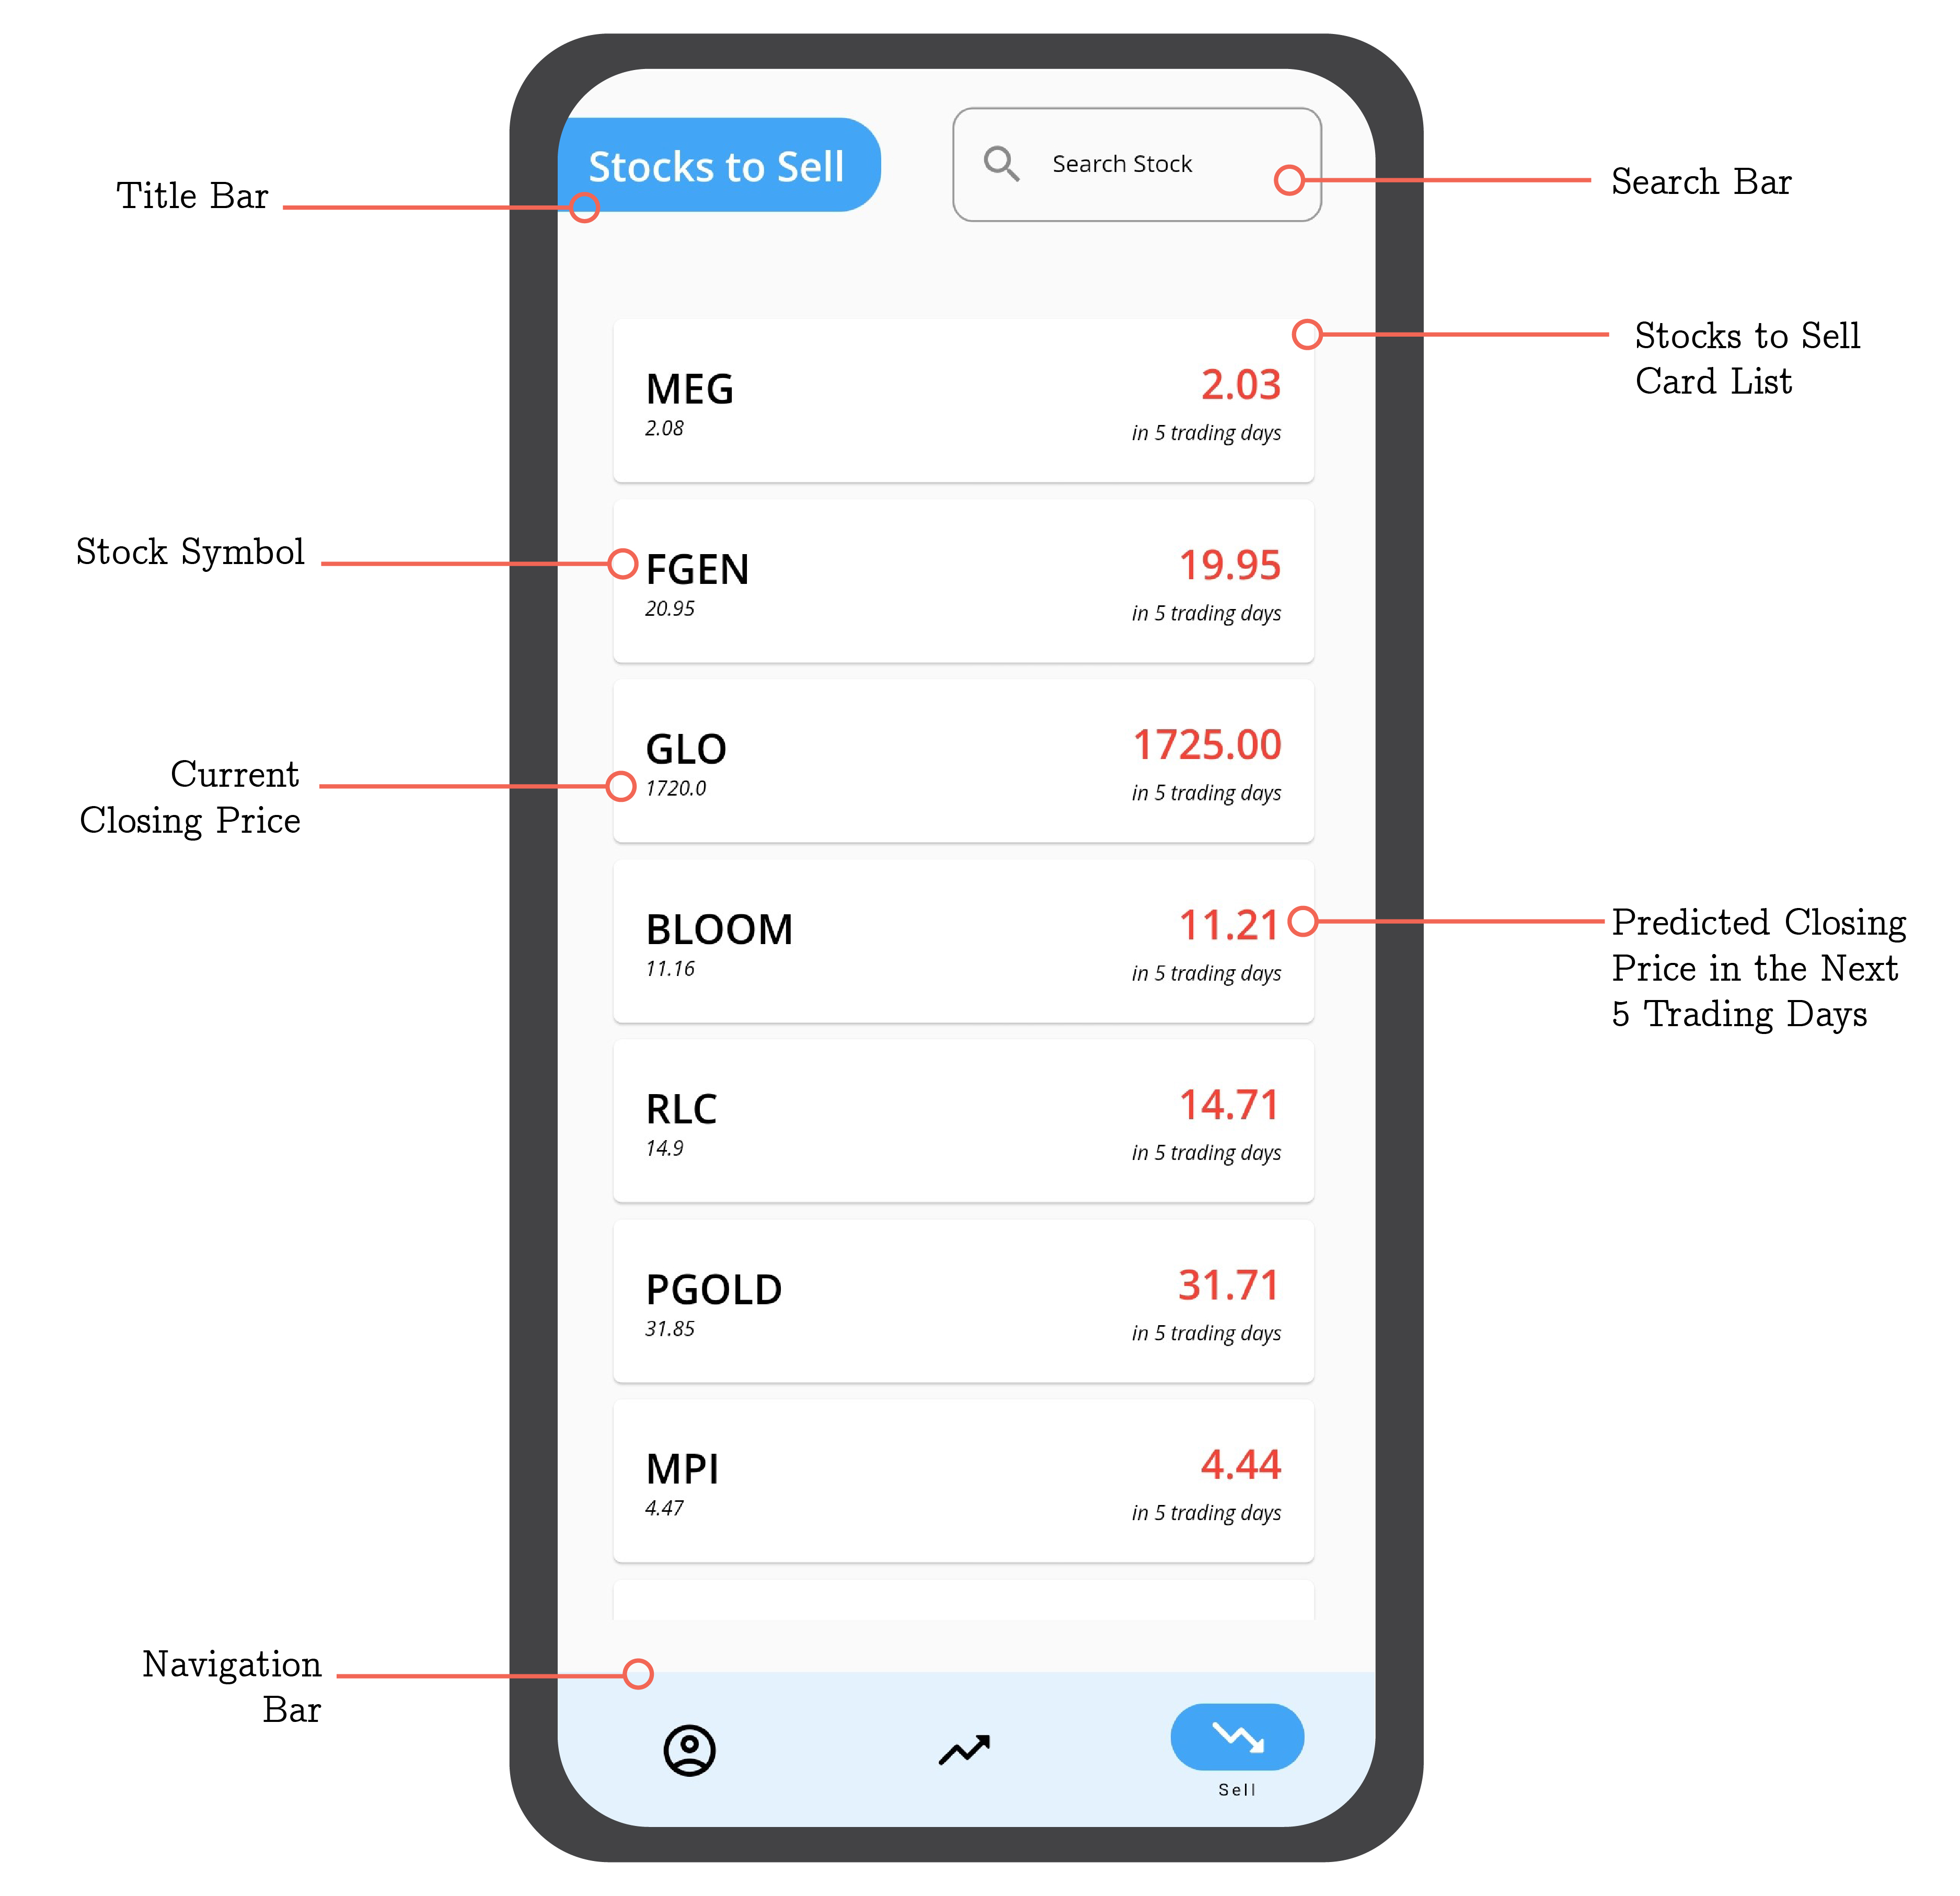
\includegraphics[height=0.40\textheight]{./assets/Chapter_4/mobile_ui/sell_ui.jpg}
  \caption{alamAPP "Sell" Screen}
  \label{fig:alamAPP_sell}
\end{figure}
\FloatBarrier


% Insert UI when a card is selected
Users have the option of tapping or selecting the listed stocks in the "Buy" and "Sell" screens 
to display additional information about the specific stock, including the predicted price graph 
of the stock (presented in Figure \ref{fig:alamAPP_predCard}), which will help users make 
decisions based on information and further reduce potential risk.
\begin{figure}[ht]
  \centering
  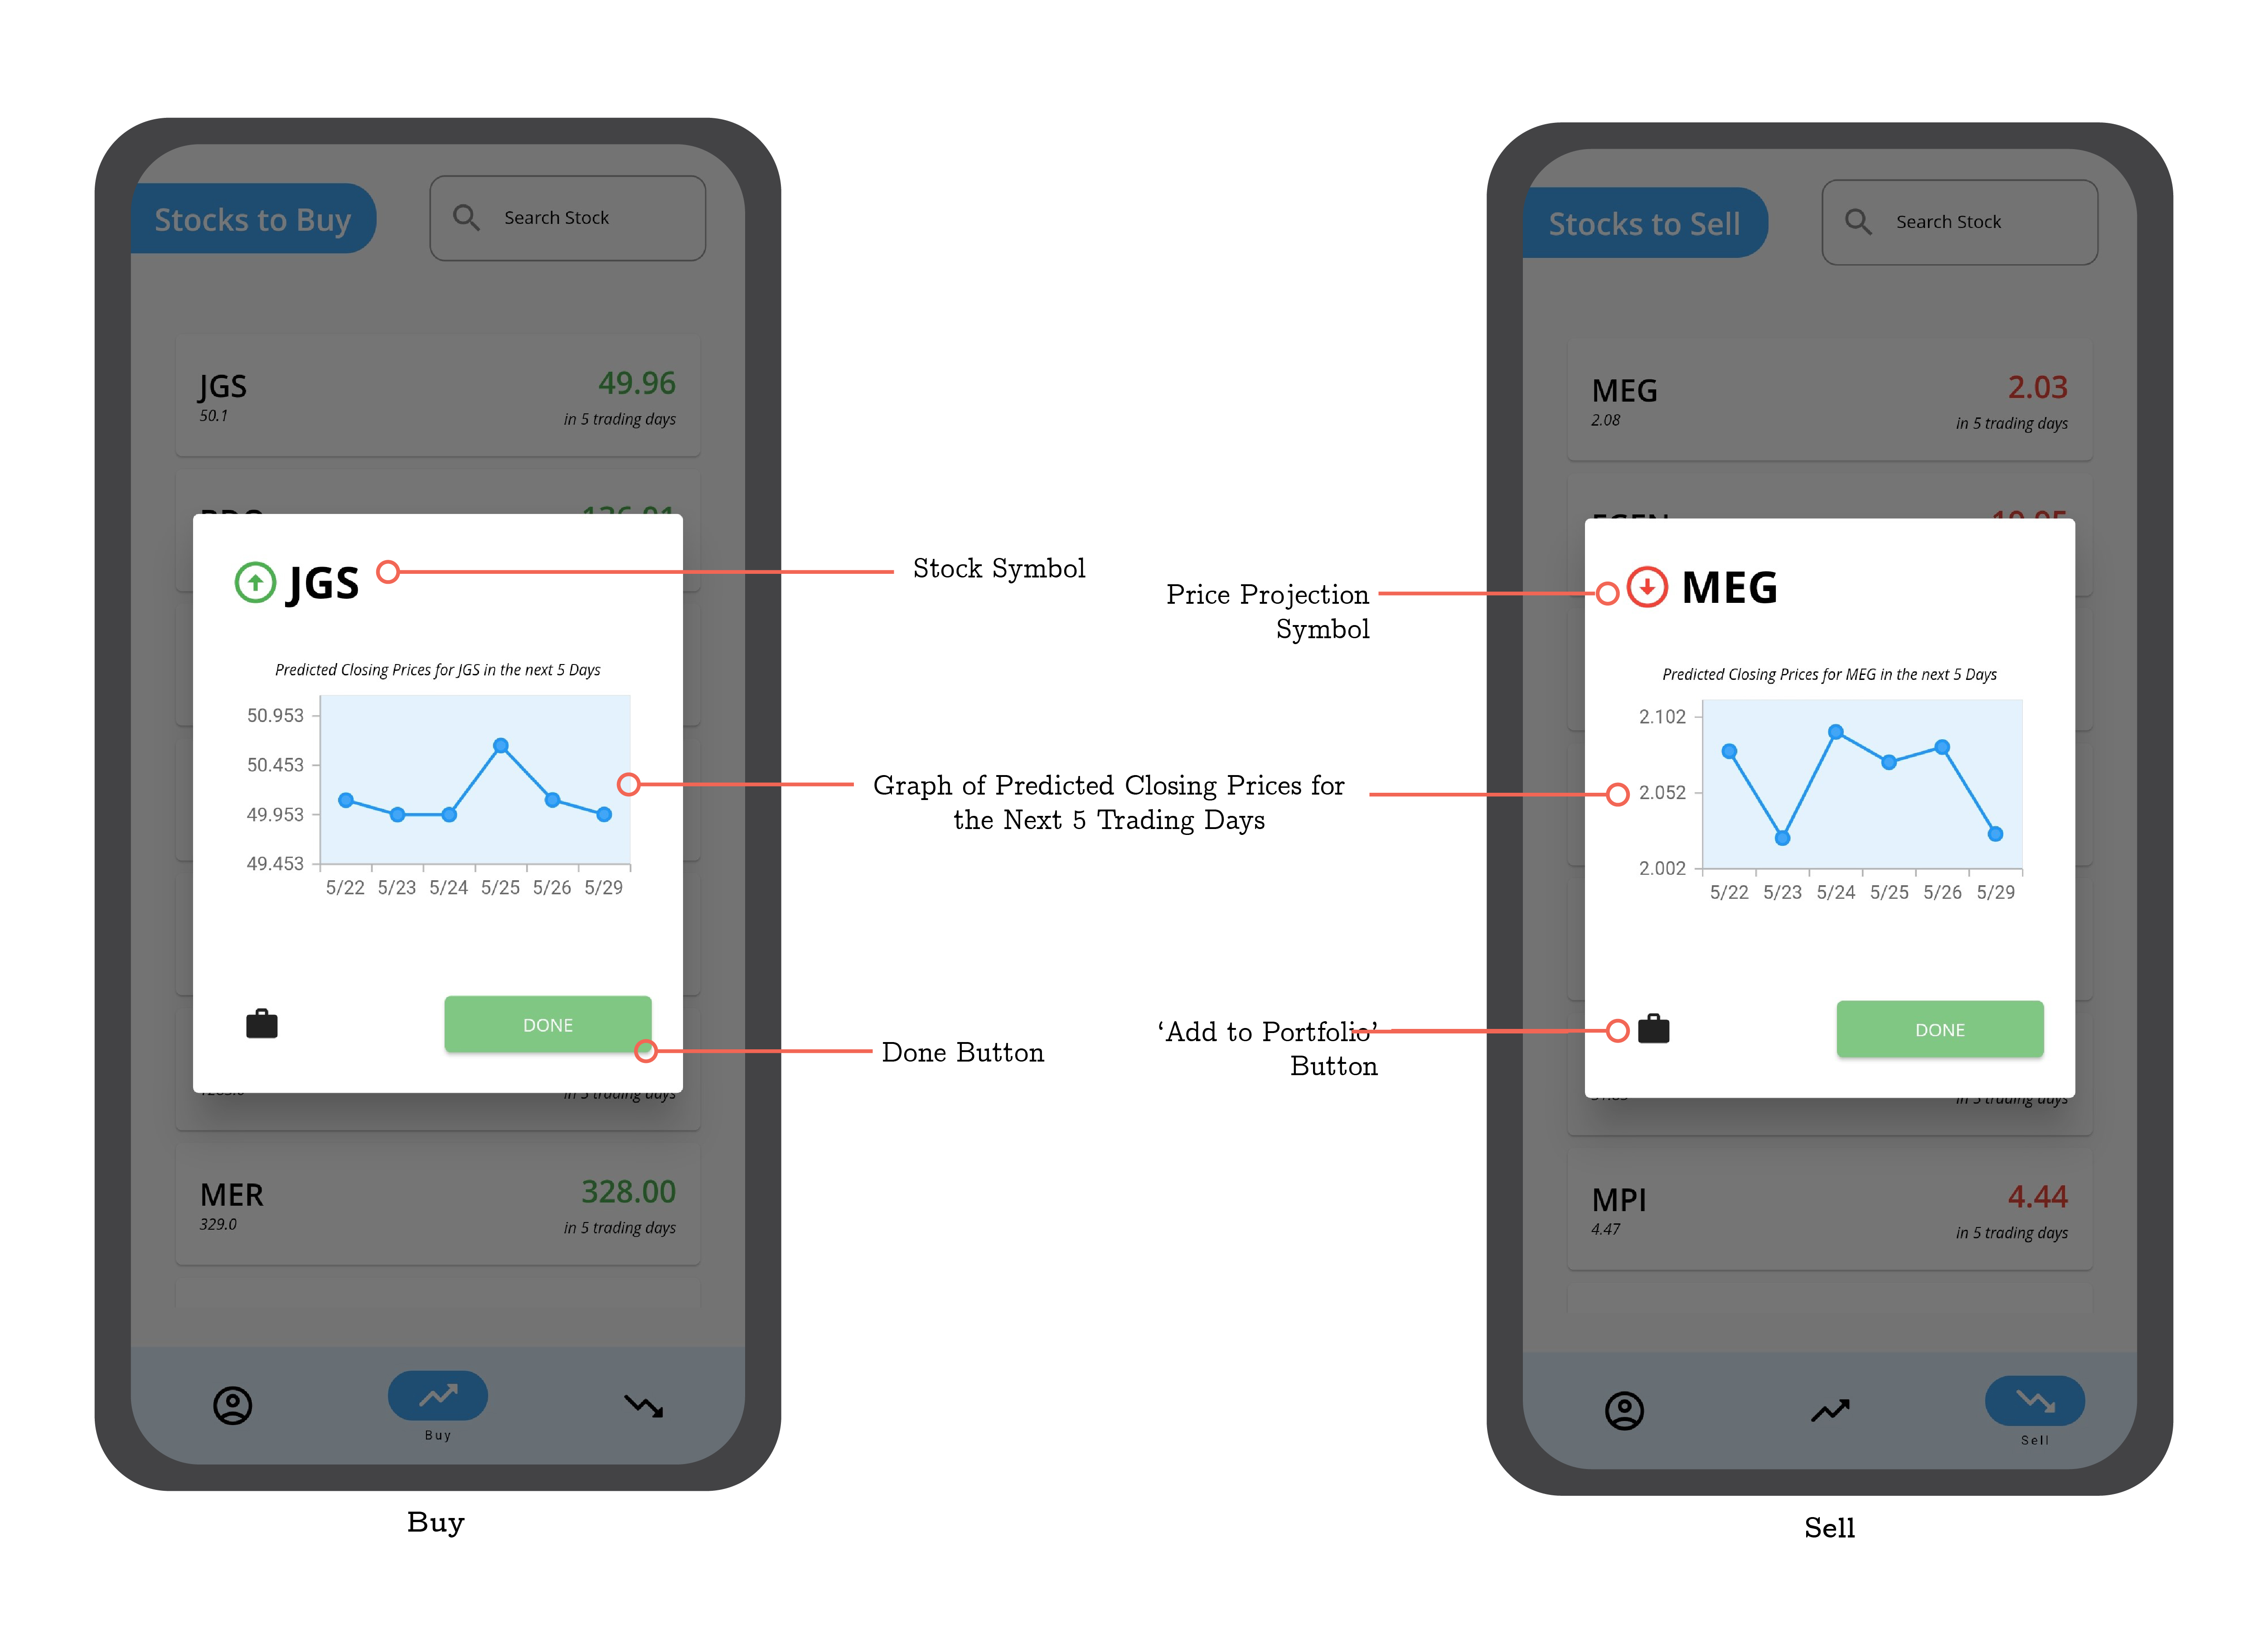
\includegraphics[height=0.40\textheight]{./assets/Chapter_4/mobile_ui/prediction_ui.jpg}
  \caption{alamAPP Prediction Graph Card}
  \label{fig:alamAPP_predCard}
\end{figure}
\FloatBarrier

Overall, the figures depicting the alamAPP's user interface 
demonstrate that the alamAPI can be used by external applications 
by connecting via the internet.

\subsubsection{Utilization of alamSYS in the alamAPP}
\label{subsubsec:utilization_alamSYS-alamAPP}
The following code snippet written in Dart, was used in the alamAPP's source 
code to get the details of the stocks to buy from alamAPI.
\textit{Note that the [reserved.domain] should be changed to
the domain address used on the alamAPI deployment}.
\hfill \\
\begin{python}
    Future<List<Stocks>> stocksToBuy() async {
        var url = 'https://[reserved.domain]/stocks_to_buy/all';
        var response = await http.get(Uri.parse(url));
        var data = jsonDecode(response.body);
        List<Stocks> stocksToBuy = [];
        if (data['Stocks'] != null) {
        data['Stocks'].forEach((v) {
            stocksToBuy.add(new Stocks.fromJson(v));
          });
        }
        return stocksToBuy;
    }
\end{python}

Meanwhile for the stocks to sell, the following code
snippet was used:
\hfill \\
\begin{python}
Future<List<Stocks>> stocksToSell() async {
      var url = 'https://[reserved.domain]/stocks_to_sell/all';
      var response = await http.get(Uri.parse(url));
      var data = jsonDecode(response.body);
      List<Stocks> stocksToSell = [];
      if (data['Stocks'] != null) {
        data['Stocks'].forEach((v) {
          stocksToSell.add(new Stocks.fromJson(v));
        });
      }
      return stocksToSell;
    }
\end{python}
